\documentclass[12pt]{article}

\input ../quiz-setup
\newcommand{\version}{} 

\newcommand{\ExamName}{Quiz \#1\version}



\begin{document}
\renewcommand{\version}{a}
\begin{minipage}{0.25\linewidth}
  \CourseName\ \Quarter \\
  \ExamName \\[1em]
  \textbf{No calculators}\\[2em]
\end{minipage}
\hfill
\begin{minipage}[t]{0.4\linewidth}
  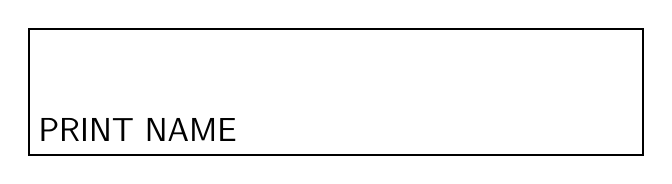
\begin{tikzpicture}[x=26mm,y=16mm]
    \draw[thick,black] (0,0) rectangle (3,1);
    \node[\faintcolor,right] at (0,0.2) {\large\textsf{PRINT NAME}};
    % \node[\faintcolor] at (1.5,0.4) {\Huge\textsf{PRINT NAME}};
  \end{tikzpicture}
\end{minipage}
\hfill
\begin{minipage}{0.25\linewidth}
  \vspace*{-2.75em}
  \ \hfill
  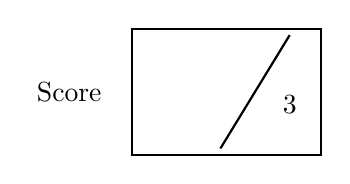
\begin{tikzpicture}[x=16mm,y=16mm]
    \draw[thick,black] (0,0) rectangle (1.5,1);
    \node at (-0.5,0.5) {Score};
    \draw[thick,black] (0.7,0.05) -- (1.25,0.95);
    \node at (1.25,0.4) {$3$};
  \end{tikzpicture}
\end{minipage}
% \medskip
\vspace*{-0.45in}

\begin{minipage}{0.45\linewidth}
  Put your answer in the 
  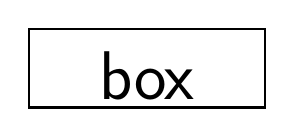
\begin{tikzpicture}[x=10mm,y=10mm,baseline=3mm] 
    \draw[thick,black] (0,0) rectangle (3,1);
    \node[\faintcolor] at (1.5,0.4) {\Huge\textsf{box}};
  \end{tikzpicture}
  provided.
\end{minipage}
\hfill
\begin{minipage}{0.5\linewidth}
  \textbf{TA:}\ 
  \parbox[t]{0.85in}{%
    \checkbox\ \TAOne \\
    \checkbox\ \TATwo  \\
    \checkbox\ \TAThree
  }
  % \ 
  % \parbox[t]{4in}{%
  % \textbf{Section Time:}
  \hspace*{0.35in}
  % \ 
  % \parbox[t]{4in}{%
  % \textbf{Section Time:}
  \textbf{Time:}
  \parbox[t]{0.55in}{%
    \checkbox\ 8am \\
    \checkbox\ 5pm
  }
  \quad
  \parbox[t]{0.55in}{%
    \checkbox\ 6pm \\
    \checkbox\ 7pm 
  }
  % }
\end{minipage}
\noindent\hspace*{-2em}\rule{\textwidth+4em}{1pt}%

\begin{enumerate}
  \setcounter{problemnumber}{0}
  \Problem %\Points{3} %
  The sum of two numbers is $63$.  Three times the first number is
  four times the second.  Find the two numbers.

  \ 
  \hfill
  The numbers are
  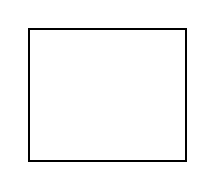
\begin{tikzpicture}[x=10mm,y=12mm,baseline={6mm}]
    \draw[thick,black] (0,-0.2) rectangle (2,1.2);
    % \node at (1.8,0.5) {\large\%};
  \end{tikzpicture}
  \ and\ 
  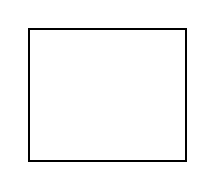
\begin{tikzpicture}[x=10mm,y=12mm,baseline={6mm}]
    \draw[thick,black] (0,-0.2) rectangle (2,1.2);
    % \node at (1.8,0.5) {\large\%};
  \end{tikzpicture}
\end{enumerate}
\newpage
\renewcommand{\version}{b}
\begin{minipage}{0.25\linewidth}
  \CourseName\ \Quarter \\
  \ExamName \\[1em]
  \textbf{No calculators}\\[2em]
\end{minipage}
\hfill
\begin{minipage}[t]{0.4\linewidth}
  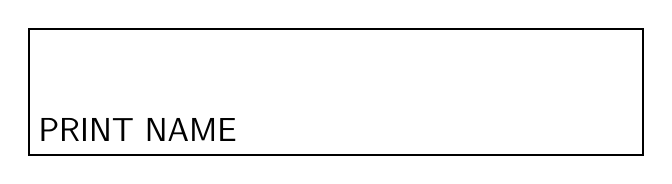
\begin{tikzpicture}[x=26mm,y=16mm]
    \draw[thick,black] (0,0) rectangle (3,1);
    \node[\faintcolor,right] at (0,0.2) {\large\textsf{PRINT NAME}};
    % \node[\faintcolor] at (1.5,0.4) {\Huge\textsf{PRINT NAME}};
  \end{tikzpicture}
\end{minipage}
\hfill
\begin{minipage}{0.25\linewidth}
  \vspace*{-2.75em}
  \ \hfill
  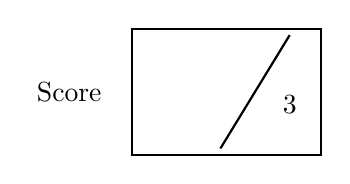
\begin{tikzpicture}[x=16mm,y=16mm]
    \draw[thick,black] (0,0) rectangle (1.5,1);
    \node at (-0.5,0.5) {Score};
    \draw[thick,black] (0.7,0.05) -- (1.25,0.95);
    \node at (1.25,0.4) {$3$};
  \end{tikzpicture}
\end{minipage}
% \medskip
\vspace*{-0.45in}

\begin{minipage}{0.45\linewidth}
  Put your answer in the 
  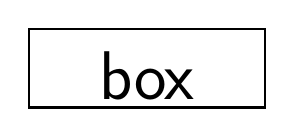
\begin{tikzpicture}[x=10mm,y=10mm,baseline=3mm] 
    \draw[thick,black] (0,0) rectangle (3,1);
    \node[\faintcolor] at (1.5,0.4) {\Huge\textsf{box}};
  \end{tikzpicture}
  provided.
\end{minipage}
\hfill
\begin{minipage}{0.5\linewidth}
  \textbf{TA:}\ 
  \parbox[t]{0.85in}{%
    \checkbox\ \TAOne \\
    \checkbox\ \TATwo  \\
    \checkbox\ \TAThree
  }
  \hspace*{0.35in}
  % \ 
  % \parbox[t]{4in}{%
  % \textbf{Section Time:}
  \textbf{Time:}
  \parbox[t]{0.55in}{%
    \checkbox\ 8am \\
    \checkbox\ 5pm
  }
  \quad
  \parbox[t]{0.55in}{%
    \checkbox\ 6pm \\
    \checkbox\ 7pm 
  }
  % }
\end{minipage}
\noindent\hspace*{-2em}\rule{\textwidth+4em}{1pt}%

\begin{enumerate}
  \setcounter{problemnumber}{0}
  \Problem %\Points{3} %
  The sum of two numbers is $56$.  Three times the first number is
  four times the second.  Find the two numbers.

  \ 
  \hfill
  The numbers are
  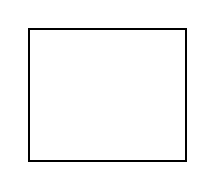
\begin{tikzpicture}[x=10mm,y=12mm,baseline={6mm}]
    \draw[thick,black] (0,-0.2) rectangle (2,1.2);
    % \node at (1.8,0.5) {\large\%};
  \end{tikzpicture}
  \ and\ 
  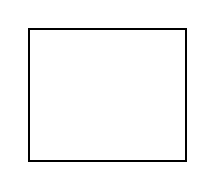
\begin{tikzpicture}[x=10mm,y=12mm,baseline={6mm}]
    \draw[thick,black] (0,-0.2) rectangle (2,1.2);
    % \node at (1.8,0.5) {\large\%};
  \end{tikzpicture}
\end{enumerate}
\newpage

\renewcommand{\version}{c}
\begin{minipage}{0.25\linewidth}
  \CourseName\ \Quarter \\
  \ExamName \\[1em]
  \textbf{No calculators}\\[2em]
\end{minipage}
\hfill
\begin{minipage}[t]{0.4\linewidth}
  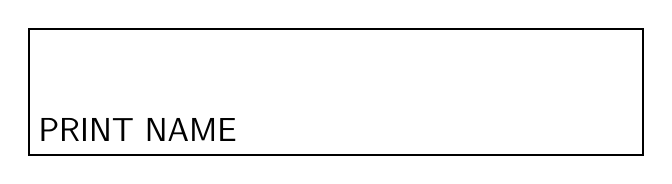
\begin{tikzpicture}[x=26mm,y=16mm]
    \draw[thick,black] (0,0) rectangle (3,1);
    \node[\faintcolor,right] at (0,0.2) {\large\textsf{PRINT NAME}};
    % \node[\faintcolor] at (1.5,0.4) {\Huge\textsf{PRINT NAME}};
  \end{tikzpicture}
\end{minipage}
\hfill
\begin{minipage}{0.25\linewidth}
  \vspace*{-2.75em}
  \ \hfill
  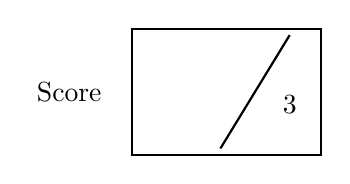
\begin{tikzpicture}[x=16mm,y=16mm]
    \draw[thick,black] (0,0) rectangle (1.5,1);
    \node at (-0.5,0.5) {Score};
    \draw[thick,black] (0.7,0.05) -- (1.25,0.95);
    \node at (1.25,0.4) {$3$};
  \end{tikzpicture}
\end{minipage}
% \medskip
\vspace*{-0.45in}

\begin{minipage}{0.45\linewidth}
  Put your answer in the 
  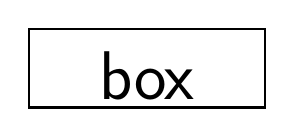
\begin{tikzpicture}[x=10mm,y=10mm,baseline=3mm] 
    \draw[thick,black] (0,0) rectangle (3,1);
    \node[\faintcolor] at (1.5,0.4) {\Huge\textsf{box}};
  \end{tikzpicture}
  provided.
\end{minipage}
\hfill
\begin{minipage}{0.5\linewidth}
  \textbf{TA:}\ 
  \parbox[t]{0.85in}{%
    \checkbox\ \TAOne \\
    \checkbox\ \TATwo  \\
    \checkbox\ \TAThree
  }
  \hspace*{0.35in}
  % \ 
  % \parbox[t]{4in}{%
  % \textbf{Section Time:}
  \textbf{Time:}
  \parbox[t]{0.55in}{%
    \checkbox\ 8am \\
    \checkbox\ 5pm
  }
  \quad
  \parbox[t]{0.55in}{%
    \checkbox\ 6pm \\
    \checkbox\ 7pm 
  }
  % }
\end{minipage}
\noindent\hspace*{-2em}\rule{\textwidth+4em}{1pt}%

\begin{enumerate}
  \setcounter{problemnumber}{0}
  \Problem %\Points{3} %
  The sum of two numbers is $49$.  Three times the first number is
  four times the second.  Find the two numbers.

  \ 
  \hfill
  The numbers are
  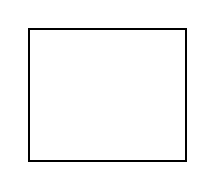
\begin{tikzpicture}[x=10mm,y=12mm,baseline={6mm}]
    \draw[thick,black] (0,-0.2) rectangle (2,1.2);
    % \node at (1.8,0.5) {\large\%};
  \end{tikzpicture}
  \ and\ 
  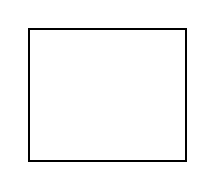
\begin{tikzpicture}[x=10mm,y=12mm,baseline={6mm}]
    \draw[thick,black] (0,-0.2) rectangle (2,1.2);
    % \node at (1.8,0.5) {\large\%};
  \end{tikzpicture}
\end{enumerate}

\end{document}
